%\documentclass[oribibl,runningheads,a4paper]{llncs}
\documentclass[a4paper]{llncs}
\usepackage{url}
\usepackage{times}
\usepackage{listings}
\usepackage{graphicx,marvosym}

\newcommand{\comment}[1]{}
\newcommand{\citenot}[1]{}
\newcommand{\blurb}[1]{{\texttt{[.. #1..]}}}


\begin{document}

\lstset{language=C,basicstyle=\small}
\lstset{numbers=left, numberstyle=\tiny, stepnumber=1, numbersep=5pt}
\lstset{tabsize=2}
\lstset{firstnumber=1}
\lstset{frame=single}
\lstset{
  language={C},
  morekeywords={assert,uchar}
}

%\mainmatter  % start of an individual contribution

%\title{Context-Bounded Symbolic Model Checking with ESBMC 1.17}
\title{Bounded Model Checking of C++ Programs using SMT Solvers}
%\subtitle{(Competition Contribution)}
%\title{TACAS'12 Competition Entry: ESBMC v1.17}
%\title{Software Verification Competition: ESBMC v1.17}
%\title{TACAS'12 Software Verification Competition: ESBMC v1.17}
%\title{System Description: ESBMC v1.17}
%\title{System Description: ESBMC v1.17 (TACAS'12 Competition version)}
%\titlerunning{}
\comment{
\author{Lucas Cordeiro$^1$ \and
	Jeremy Morse$^2$   \and
	Denis Nicole$^2$   \and
	Bernd Fischer$^2$}
\authorrunning{Lucas Cordeiro, Jeremy Morse, Denis Nicole, Bernd Fischer}
\institute{
  $^1$ Electronic and Information Research Center, %\\
  Federal University of Amazonas, Brazil\\
  %\url{lucascordeiro@ufam.edu.br}
  %\\\smallskip
  $^2$ Electronics and Computer Science, %\\
  University of Southampton, UK\\
  %\url{{jcmm106,dan,bf}@ecs.soton.ac.uk}
  %\url{http://www.ecs.soton.ac.uk}
  \url{esbmc@ecs.soton.ac.uk}
}
}

\maketitle

\begin{abstract}
Bounded model Checking (BMC) of C++ programs presents greater complexity than C programs 
due to features that the languages offers, such as templates, containers, and exception handling. 
We present ESBMC++, a bounded model checker for C++ programs, which encodes the verification 
conditions via an operational model using different background theories and passes them directly 
to an SMT Solver. This operational model is an abstract representation of the standard C++ library,
which conservatively approximates its semantics. Our experimental results show that our approach can 
handle a wider range of the C++ constructs and substantially reduce the verification time. 
\end{abstract}

%------------------------------
\section{Introduction}
%------------------------------
%
Bounded model checking (BMC) has already been successfully applied to
verify software and to discover subtle errors in real
systems~\cite{handbook09}.\ In an attempt to cope with growing 
system complexity, Boolean Satisfiability (SAT) solvers are increasingly 
replaced by Satisfiability Modulo Theories (SMT) solvers to prove the generated 
verification conditions (VCs)~\cite{Armando09,Ganai06,Cordeiro12}.\
There have also been attempts to extend BMC to the verification of C++ 
programs~\cite{Blanc07,Florian12}. The main challenge here is to handle large 
programs and support the features that the languages offers, such as templates, 
containers and exception handling.

The verification of C++ programs is an important topic due to the fact that there are 
several real-world applications that use C++ as its mainstream programming 
language, which includes software/hardware verification tools, information retrieval 
machines, databases, simulators, embedded systems, and telecommunication systems. 
If we compared the C++ to the C programming language, C++ arises much more challenges 
since it provides a wider set of features, libraries and functionalities that would require 
too much effort to develop from scratch. These features include object-oriented programming 
(OOP), specialized input-output libraries (e.g., stream libraries), and the template usage 
(including STL containers, which have the most popular data structures in Computing Science).

Systems that make use of the C++ language (and its functionalities) tend to require a high 
verification effort since the errors are hard to find as its own structure grows. 
To hunt bugs in C++ applications, a verification tool has deal with crucial characteristics 
(e.g., speed, accuracy, efficiency, and friendliness) to make it attractive to be used in the 
mainstream software development. Obviously, if the C++ programming language seems to be a more 
complex version than C, then its verification will be more complex as well. To tackle this problem, 
our proposed approach applies Bounded Model Checking (BMC) to C++ programs using an operational model 
of the C++ libraries. This operational model is an abstract representation of the standard C++ library,
which conservatively approximates its semantics. In particular, we focus on the STL sequential containers 
operational model, its preconditions and simulation features (e.g., how we store the elements values 
of the containers and intern class methods), and how these are used to verify the C++ programs.

\section{Background}
%
Background here (Lucas)...

\section{C++ Operational Model}
%
During the verification process, ESBMC needs to identify all the features and specifications of the code in order to generate the AST. 
In case of the C++ code, the basic representations (e.g., features related to object orientation, template and exception handling) are 
set internally to ESBMC in different levels (typecheck, goto-program, and goto-symex). However, ESBMC must have the specifications 
related to definitions of C++ libraries such as classes, methods, and types. Keeping this in mind, we developed a simplified representation 
of C++ libraries, with their respective classes, methods, and other features, called C++ Operational Model (COM).

The development process of the COM can be divided into two phases: structural and modeling. In the structural phase, we built a set 
of classes with a specific hierarchical relationship and the signature of their methods and specific data, which consequently resulted 
in a simplified structure representing the set of C++ libraries. From this structure, we modeled the methods of each class and this 
modeling is focused for the validation and verification of all properties that include the specific method.
%

\subsection{Structure and Model}
%
In general, the verification process of a program ESBMC can be divided into two segments, respectively, identifying the expressions and 
verifying all properties related to those expressions, and in the identification step, the ESBMC must support all syntactic features 
of the language in which the program is implemented. Based on this, we have adopted two approaches to the development of the support 
of all syntactic characteristics of a C++ code. The first is to identify the basic structures of language, for example, polymorphism 
and template, modifying the kernel of the tool so that the AST can contain all the necessary information to verify these structures. 
The second approach is directly related to the definitions (classes, methods, functions, types) present in the C++ libraries, the goal 
is to build an operational model so that the ESBMC can rely on it to identify such definitions and also, verify all the properties related 
to these definitions based on the implementation of this model. It is important to say that this model is inserted into the verification 
process at the level of source code, ie, both model and source code are passed as parameters at the beginning of the verification process, 
so that the scan, parser and typecheck are done with the purpose of creating the AST joining the implementations.

The first step of the construction process of this operating model is the formation of a simplified structure,
which should get closer to actual structure as possible. This way, based on the documentation of the language C++
[1] the set of libraries was divided according to their functionalities, into four subsets called C Libraries,
Input/Output Stream, Standard Template Libraries, and General Libraries, respectively. Each library present in a
subset is particularly related to the other libraries, not only in its functionality but also in its structure due
to the fact that many libraries depend on definitions of others. From this, we performed an analysis in the respective 
subsets, Figure \ref{figure:cpp-diagram}, such a way that could be identified dependencies between each library and thus develop a simplified 
structure of each. The topics that follow describe the structure of subsets of libraries shown in Figure \ref{figure:cpp-diagram}.
%
\begin{figure*}[ht]
\centering
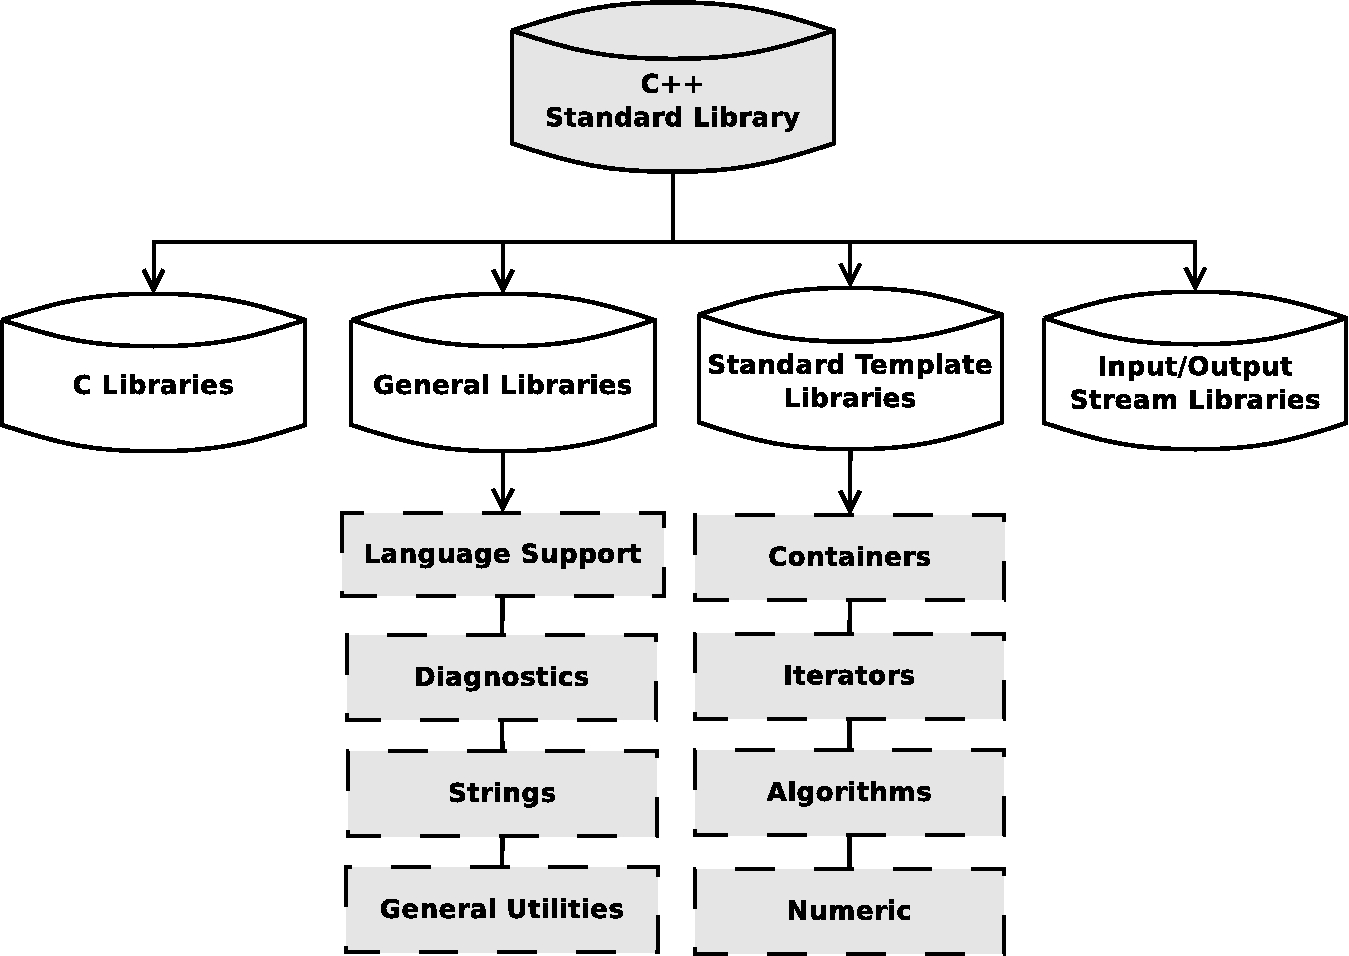
\includegraphics[scale=0.28]{figures/diagramascpp.jpg}
\caption{Representation of the configuration and functional classification of the operational model.}
\label{figure:cpp-diagram}
\end{figure*}

\subsection{C Libraries}
%
The C++ Standard Libraries also includes all the ANSI-C libraries, seeing that it's an extension of this language. The ESBMC 
supported language ANSI-C, however when occurred verification in C++ code; the same follow one different way for kernel's tool, 
passing for a specific typecheck directed to C++ software. For this reason, it's also necessary to build a representation of 
the ANSI-C libraries' set in the operational model. Meantime, we can define this libraries' set in simplified structure 
consisting of macro definitions and functions. Among the ANSI-C libraries' set exist libraries containing only macro definitions, 
for example, the ciso646 library that define a spelling set to the logic operators. To build the structure of this library, we 
distingue two kind of spelling: we define the macro set $M$ and operators set $O$. For convention, we assume 
$\left\{and, \: and\_eq, \: bitand, \: bitor, \: compl, \: not, \: not\_eq, \: or, \: or\_eq, \: xor, \: xor\_eq\right\} \subset M$, and 
$\left\{
\: \&\&, 
\: \&= \:, 
\: \& \:, 
\: | \:, 
\: \widetilde{} \:, 
\: ! \:, 
\: || \:, 
\: |= \:, 
\:\: \widehat{} \:\:, 
\: \widehat{}= \: 
\right\} \subset O$. 
Therefore, we define the syntax for these definitions set as:
\\
\begin{equation}
\left( \alpha \in M \wedge \beta \in O \right) \rightarrow 		          \left(\forall\alpha\right)\left(\exists\beta\right)\left(\alpha\equiv\beta\right)
\label{eq:csi646-definitions}
\end{equation}
\\
Within the ANSI-C libraries set, also we can represent the structure of others libraries with functions only. This is case of the 
csignal library that dealing with signals emitted in a given code. Basing in this concept, we define that the operational model of 
this library has been represented to signal and raise functions, respectively, and furthermore, to vector $v_{i}$ assuming that 
$\left\{ i \in \aleph \:|\: 0 \leq i \leq 15 \right\}$ and to finite signals set $A$ assuming that 
$\left\{2, 4, 6, 8, 11, 15\right\}\:\subset\:A$. The functional signal records certain function in one specific signal such 
that when the function raise is called with the respective signal the registered function is called, therefore, 
assuming $f$ as a un-deterministic function and as null element, is obtained following the formalize modeling.
\\

\begin{equation}
\label{c-csignal}
C := \left [ \begin{array}{ll} 
                \left(\varphi \subset A\right) \\
                \wedge \, \, \left(2 \leq \varphi \leq 15\right) \\
                \wedge \, \, \left(f \neq \phi\right) \\
              \end{array} \right ]  \\ 
\end{equation}

$\newline$

\begin{equation}
\label{p-csignal}
C := \left [ \begin{array}{ll} 
                \left(i_{0} = \varphi\right) \, \, 
                \wedge \, \, \left(v_{i} = f\right)\\
              \end{array} \right ]  \\ 
\end{equation}
\\
The code section that represents this structure can be observed in the following.

\begin{figure}[ht]
\centering
\begin{minipage}{0.7\textwidth}
\begin{lstlisting}
#ifndef STL_CSIGNAL
#define STL_CSIGNAL
typedef void (*sighandler)(int);
sighandler vetor[16];
  void signal(int sig, sighandler func);
  int raise(int sig);
#endif
\end{lstlisting}
\end{minipage}
\caption{Structure of the CSIGNAL.}
\label{figure:structure-of-the-CSIGNAL}
\end{figure}

\begin{figure*}[ht]
\centering
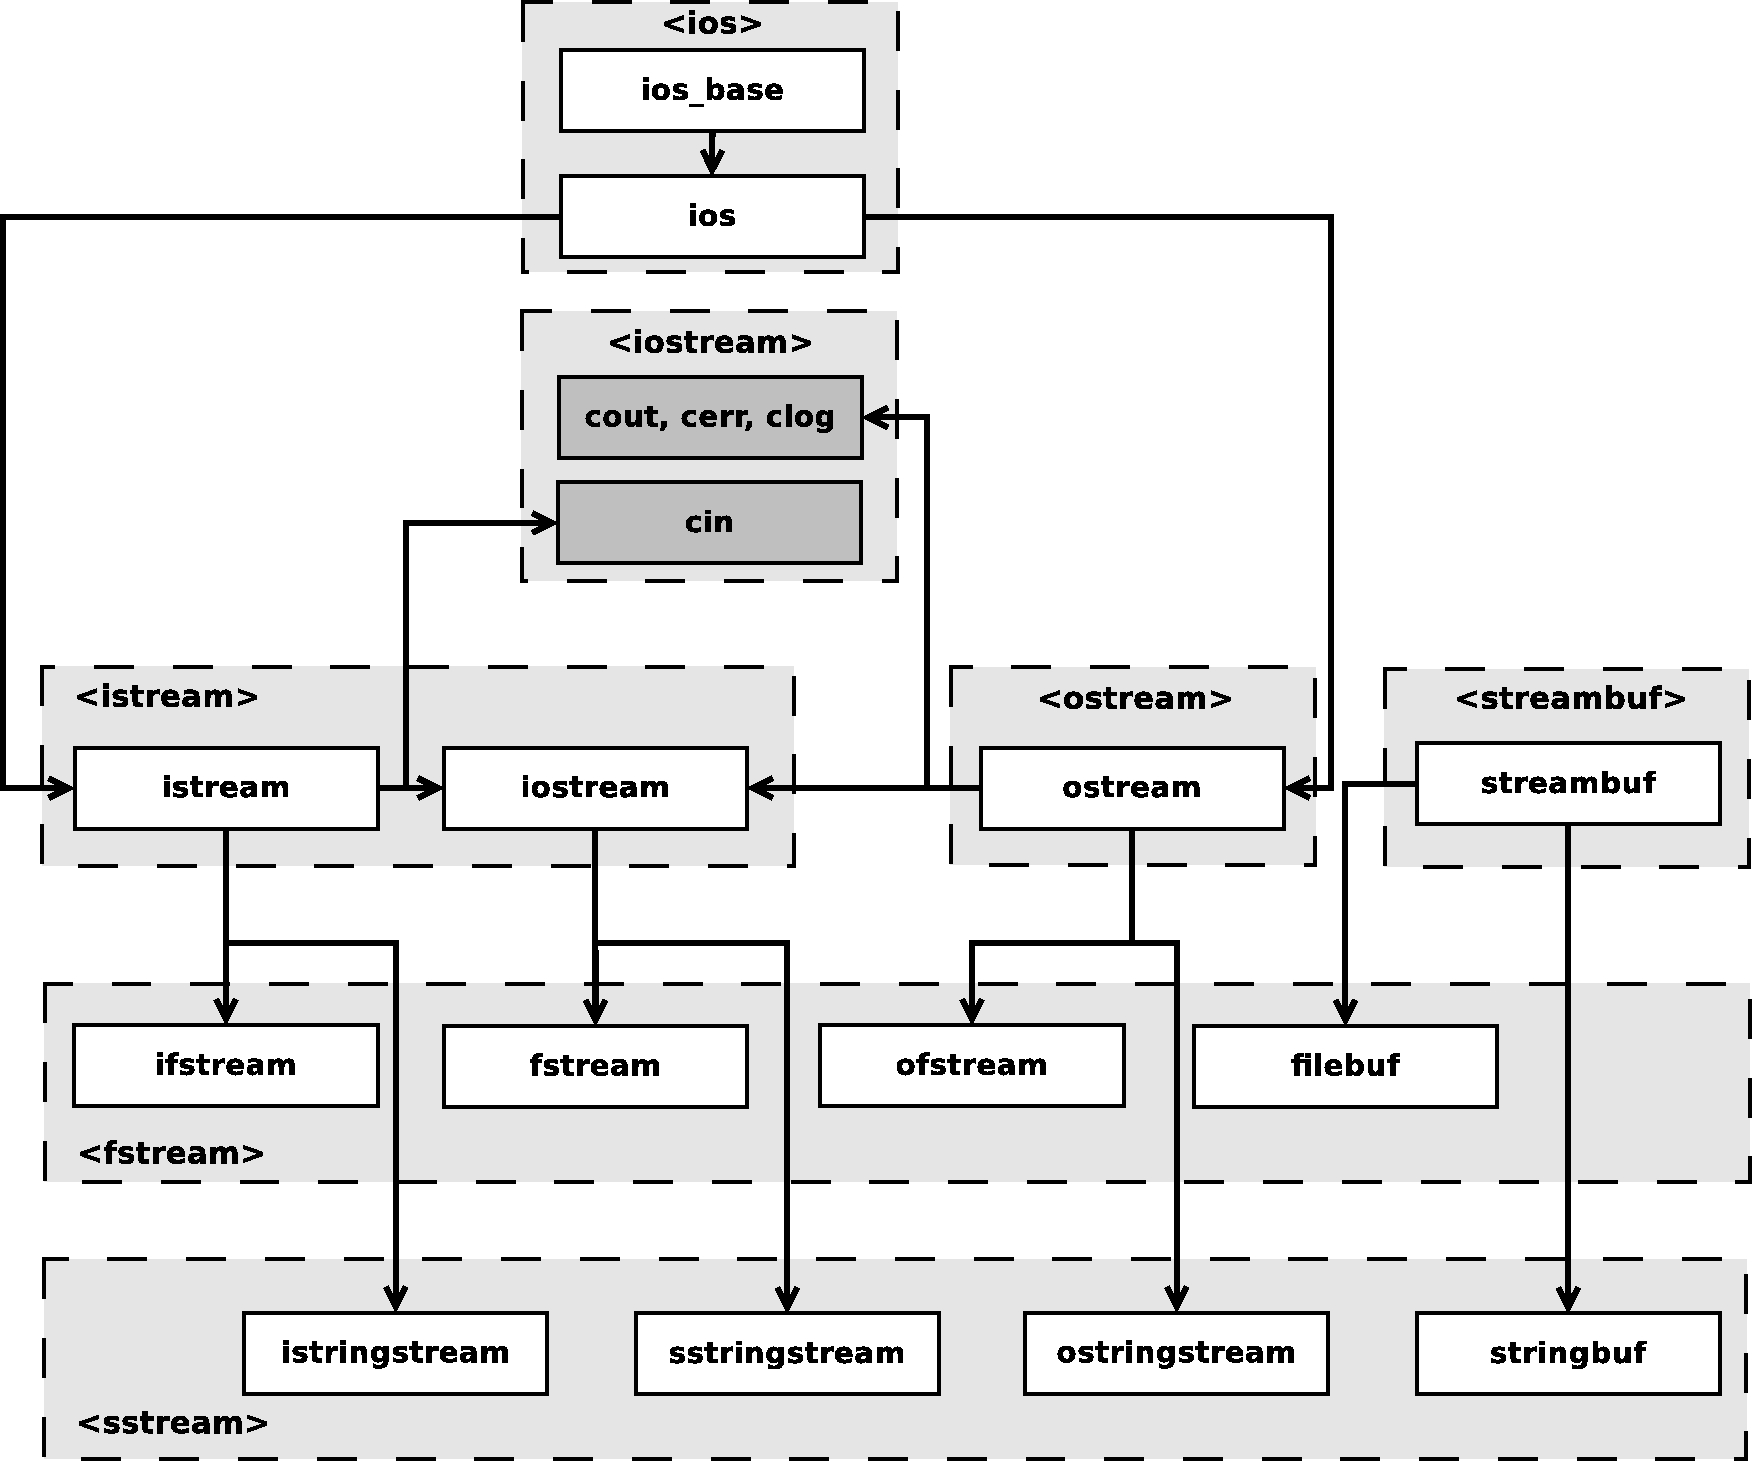
\includegraphics[scale=0.22]{figures/inputoutputdiagram.jpg}
\caption{Diagram about hierarchical structure of the Input / Output Stream Libraries.}
\label{figure:cpp-inputoutputdiagram}
\end{figure*}

\subsection{Input / Output Stream Libraries}
%

The libraries group related to flow control of input and output data inside to certain program is represented for the libraries set 
called Input / Output Stream. Aiming to build the operational model of this set, we elaborated a hierarchical structure really similar 
to real that can be observed in Figure \ref{figure:cpp-inputoutputdiagram}.
\\
%to do formalization
\\

\subsection{Standard Template Libraries}

This set is subdivided in four categories: Containers, Algorithms, Iterators and Numeric. The algorithm library is the only one that 
composes the Algorithms categories and it has a model formed by 66 functions that present as main objective the manipulation of STL 
containers. Therefore, we define the variables set $It$ representing ranges and $Val$ representing any values, we assume 
$\left\{it_{1}, it_{2}\right\} \:\subset\:It$ and $\left\{n\right\} \:\subset\:Val$. From this, we can exemplified the functionalities 
of this library through the model's find function that search between the range compose to $it_{1}$, pointed to the first element 
of range, and $it_{2}$, pointed to the last element of range, the value represented to $n$. The modeling of this function has the 
following formal representation:
\\
%to do formalization
\\
The Numeric category present the numeric library formed by four functions that manipulated numeric sequences basically. 
To exemplified the functionalities of this library, we take as exempla the accumulate function; it covers a certain range adding 
the values inside the same in one variable (accumulator). Keep this in mind, we assume $\left\{it_{1}, it_{2}\right\} \:\subset\:It$ 
and $\left\{n\right\} \:\subset\:Val$, obtaining the modeling following:

\subsubsection{Structure.}

In this session, we will focus on the STL sequential containers operational model, its preconditions and simulation features (like how we store the elements values of the containers and intern class methods), and how this is used to verify a C++ program code.

	The structure of STL containers is based on the C++ structure itself, including its classes, operators, methods, functions and intern variables. It is divided in: iterations, capacity, element access, modifiers and unique members. As the containers structure differs a little between each other, some of their methods will vary too, changing its intern model as well. For example, a list container does not have a reference operator (operator[]), and the elements are reached only by iterators (list has a dynamic structure, unlike deque or vector). Lists also have unique methods, optimized by its dynamic structure, like merging, elements sorting, reverse order, etc.
	Vector also have unique methods, related to size and capacity manipulation, and it also does not have push\_front() and pop\_front() methods. Further information can be reached in C++ Reference website (www.cplusplus.com/reference/stl).

	
\subsubsection{Model Semantics.}
	
	Let us consider that a container model is composed by five types of variables, \emph{I}, \emph{C}, \emph{N}, \emph{P} and \emph{T}. \emph{I} represents a iterator that points to a position in the container, \emph{C} represents the container itself, N represents natural integer numbers used in the container, like size, capacity and elements index, \emph{P} represents the memory address where \emph{T} is located, and \emph{T} represents de values stored in the container. For convention, we assume that \emph{\{c, v, d, l\}} $\subset C, \{i, j, n\} \subset N$ and $\{it1, it2\} \subset I$. 
	
	
	The containers contain an array of elements \emph{T}, and their positions in the memory are represented by pointers \emph{P}.
Assuming this, the syntax for integer expression is:
%
\[\begin{array}{r@{\:\:}c@{\:\:}l}
\\[-5ex]
\mathit{Int}  & ::= & \: \mathit{N} \: | \: \mathit{Z} \: | \: \mathit{C.size} \: | \: \mathit{C.capacity} \: | \\
              &     & \: \mathit{Int} ( + \: | \: ? \: | \: * \: | \: ...) \mathit{Int}  \: | \\
              &     & \: \textit{It} ( + \: | \: - ) \textit{It} 
\end{array}
\]
%
Where variables included in the containers like \emph{size} and \emph{capacity} return a integer value, as the arithmetics operations between integer values. 
Similarly, the syntax for iterator expressions is:
%
%
\[\begin{array}{r@{\:\:}c@{\:\:}l}\label{iterator-semantics}
\\[-5ex]
\mathit{It}   & ::= & \: \mathit{I} \: | \: \mathit{It} ( + \: | \: - ) \mathit{It} \: | \: \mathit{C.begin} \: | \: \mathit{C.end} \:  \\
\end{array}
\]
%
Where \emph{begin} and \emph{end} are methods that returns iterators pointing to the beginning or the end of a container. We also have iterator operations that returns iterators too. 
For \emph{P} (memory address values), the syntax is as follows:
%	
\[\begin{array}{r@{\:\:}c@{\:\:}l}\label{pointer-semantics}
\\[-5ex]
\mathit{P}  & ::= & \: \mathit{p} \: | \: \mathit{It.pointer} \: | \: \mathit{C.array} \: | \\
            &     & \: \mathit{It.source} \: | \: \mathit{P}  ( \: + \: | \: - \: )  \textit{P} \: \\
\end{array}
\]
%	
Where \emph{pointer} is a memory address that stores the element in the container pointed by the iterator, \emph{array} is another memory address marks the beginning of the container, \emph{source} is the address that makes the link between the iterator and its pointed container (stores the container \emph{array} value). There is also the pointer return from pointer operations.
The syntax for \emph{T} values is the following: 
%
\[\begin{array}{r@{\:\:}c@{\:\:}l}\label{element-semantics}
\\[-5ex]
\mathit{T}   & ::= & \: \mathit{t} \: | \: \mathit{*It} \: | \: \mathit{*P} \: | \: \mathit{C_n} \:  \\
\end{array}
\]
%
Where \emph{*It} is the value stored in the position pointed by a iterator \emph{It}, similarly \emph{*P} is the value stores in the \emph{P} position of the memory, and $\mathit{C_n}$ is a element of a container \emph{C} in the position \emph{n}.
%
\comment{
To test the assertions, we use Booleans expressions, with the following syntax: 
%

\[\begin{array}{r@{\:\:}c@{\:\:}l}\label{boolean-semantics}
\\[-5ex]
\mathit{Bool}  & ::= & \: \mathit{Int} ( < \: | \: > \: | = \: | \: ... ) \mathit{Int} \: | \\
               &     & \: \mathit{It} ( < \: | \:> \: | \: = \: | \: ... ) \mathit{It}  \: | \\
               &     & \: \mathit{T} \: = \: \mathit{T} \: | \: \neg\mathit{Bool} \: | \\
               &     & \: \textit{Bool} ( \vee \: | \: \wedge | \: ... ) \textit{Bool} \: \\
               
\end{array}
\]
}
\subsubsection{Model.}
	To simulate appropriately the containers, our model makes use of three variables: a variable \textit{P} called array, that points to the first element of the elements array, a natural value size, that stores the quantity of elements in the container, and a natural value capacity, that stores the total capacity of a container (valid onliy for vectors). Note that, as the elements are added in the container (specifically in vectors) and the size grows, the capacity also grows at a rate of 2*size, every time the size reaches the capacity value.
	Similarly, iterators are modeled using three representing variables: a variable P called pointer, which contains the memory address to the correspondent element \textit{T} in the container, a variable N called position, which contains the index value pointed by the iterator, in the container, and a variable P called source, which contains the memory address correspondent to the first element \textit{T} stored in the container.
	The vector container model has a structure as it follows:
	
	\[\begin{array}{r@{\:\:}c@{\:\:}l}\label{container-model}
\\[-5ex]
\ &  &\: \mathit{C} = \{ \mathit{P}, \mathit{C.size}, \mathit{C.capacity}\} \:
               
\end{array}
\]
	
	Where \textit{P} is a memory address where it is stored the elements of the container, \textit{C.size} is the total number of elements in the container, and \textit{C.capacity} is the total capacity of the vector, simulated internally in the model.
	The main methods of a vector (and sequential containers, in general) have only three types of operation: insertion, exclusion and search. Methods like \textit{push\_back()}, \textit{pop\_back()}, \textit{front()}, \textit{back()}, \textit{push\_front()} and \textit{pop\_front()} are only a simplified variation of those main methods, optimized for some containers (like popping the last element of a stack).

	%An insert method is represented by the following structure:
	In order to represent the model, consider a container $C\{cont\}$, with a method $cont.insert \rightarrow It$ that returns a iterator result and makes use of a iterator $It\{position\}$, pointing to the desired insertion position, a template value $T\{value\}$ with the element to be inserted and a integer $N\{quantity\}$, that informs the amount of elements to be inserted in the desired position.\\
	
\[\begin{array}{r@{\:\:}c@{\:\:}l}\label{insert1-model}
\\[-5ex]
	 & &	cont.insert(position, value, quantity) \Longrightarrow  \\
	 &   &	\: \: \: cont'.size = cont.size + quantity \\
	 &   &	\: \: \: *(position + N\{0, ... ,quantity\}) = value \\
\end{array}
\]
	There is also another way to represent the insert method. It is possible to insert a sequence of elements in the desired insertion position, using both iterator or pointer bounds. For this, consider a iterator $It\{first\}$, marking the first element to be inserted, and another iterator $It\{end\}$, pointing to the first element after the end of the sequence to be inserted in the required position. Therefore, we have:\\

\[\begin{array}{r@{\:\:}c@{\:\:}l}\label{insert2-model}
\\[-5ex]
	 & &	 cont.insert(position, first, last) \Longrightarrow \\
	 &   &\: \: \: cont'.size = cont.size +( last - first) \\
	 &   &\: \: \: *position = *first \\
\end{array}
\]

	The same model above is valid for pointers $P\{first\}$ and $P\{last\}$. This kind of insertion (with pointers) does not return a iterator.
\\
%
	%Similarly, an erase method is structured like the following:\\
	The erase method works similarly to the insert method. It also uses iterator positions, integer values and pointers, but does note uses values, as the exclusion is made by a given position, regardless the value. It also returns a iterator position, pointing to the position next to the previously erased part of the container. The next model shows a erase method that excludes a single element:\\
%

\[\begin{array}{r@{\:\:}c@{\:\:}l}\label{erase1-model}
\\[-5ex]
\
	& & \mathit{cont.erase} (\mathit{position}) \Longrightarrow\\
	&  & \: \: \:	\mathit{cont'.size} = \mathit{cont.size} - \mathit{1}\\
	&   & \: \: \:	\mathit{position'} = \mathit{position} + \mathit{1}\\
\end{array}
\]
	It is also possible to exclude a number of elements from the container, marking the bounds with iterators. Works similarly to the equivalent insert method:\\

\[\begin{array}{r@{\:\:}c@{\:\:}l}\label{erase2-model}
\\[-5ex]
	& &  \mathit{cont.erase} (\mathit{position}, \mathit{first}, \mathit{last}) \Longrightarrow\\
	&   & \: \: \:	\mathit{cont'.size} = \mathit{cont.size} -(\mathit{last} - \mathit{first})\\
	&   & \: \: \:	\mathit{position'} = \mathit{last}\\
\end{array}
\]

	Searches are made in a container by using reference operators and a pointing type (pointer or iterator), and return the reference value (the element stored itself). It can be considered as values $N\{*It\}$, $N\{*P\}$ or $N\{\mathit{C_n}\}$ \\

	The structure of iterators is treated differently from the other types. The model is the following:\\
	\[\begin{array}{r@{\:\:}c@{\:\:}l}\label{iterator1-model}
\\[-5ex]
 \ &  &\: \mathit{It} = \{ \mathit{pointer}, \mathit{pos}, \mathit{cont\_pos}\} \:\\
               
\end{array}
\]
	
	Where \textit{pointer} is a memory address that points to the real position of the required element in the container (pointed by the iterator), \textit{pos} is the iterator index internally in the container, and \textit{cont\_pos} is a memory address equivalent to \textit{cont.array}, being cont the container pointed by the iterator.

%
\subsection{General Libraries}
%
The libraries that performing more specific functions in the context of the C++ Standard
Libraries have been defined as General Libraries and are subdivide in four particular categories:
Language Support, Diagnostics, Strings and General Utilities.
The Language Support category is compose by four libraries that work respectively with
exception handling (exception), types information (typeinfo), dynamic allocation of memory (new) and 
numeric limits (limits). Each library contains an structure formed by classes, specific types, methods
and functions, however the limits library is one exception, seeing that it implements the definitions
related to numeric elements, therefore, your structure is formed by one class with the numeric
elements definitions and eight functions for manipulate this elements. A lot of functionalities related to
exception handling, dynamic allocation of memory and types information have been implement in the
ESBMC's kernel, however is important to have one representation about the libraries relationship to
this functionalities so that tool is capable of identify all methods and definitions related to same.

The stdexcept library is the only one the form the Diagnostic category, seeing that it
implements kind of standard exceptions divide in two subcategories: logic errors and runtime errors. To build it model, we defined the exception set 
$E$ assuming that $\left\{logic, domain, invalid\_argument, length, out\_of\_range, runtime, range, overflow, underflow\right\} \subset E$, 
being that represent an element within to set $E$ such that for each $e_{i}$exist
one class $\varphi(e_{i})$ that represent it, being that all $\varphi(e_{i})$ conatins one construtor that define a message contains a
constructor that sets a message to be thrown if there is of these errors in the program. Whenever one
of the constructors of these classes is called, one $assert(0)$ is throwing, forcing the ESBMC to identify this
error and report it in the counterexample. A hierarchical representation of the model can be observed
in Figure 5 and the formalization of the same in Figure 6.

The General Libraries category also includes definitions about the manipulation of characters sequences, such definitions are implemented in 
the library string. In the model constructed to represent this library, we implemented it structure through the class called string that contains 
the main features of the library, and the iterator class containing the representation of the iterator for strings. In general, we define the 
string object as an array of char, so that all heuristics that must be observed in handling vectors are therefore approached in this model. 
From of the principle that main operations implemented by this library are restricted to creation, insertion, deletion and search of elements 
inside to object string, we take as example the creation and search operations to exemplify and formalize the model created for this library. 
Therefore, firstly we assume $S$ as the set of string variables, $c$ as character non-deterministic, the set $\left\{n, i, pos, length\right\} \subset N$, 
and we define that s representing a string, the same has two attributes: the string size described by $length$, and a character sequence that 
represent it described by $str_{i}$, such that $i$ represent the position of some character inside to string. Keep this in mind, can be defined a 
constructor method that creates a string containing $n$ times the character $c$ and, furthermore the find method that search a character within a 
certain string from a given position described by $pos$. Such formalizations can be observed in the following.

\begin{equation}
\label{cconstructor-string}
C := \left [ \begin{array}{ll} 
                \bigvee^{n}_{j=0} str_{j} = store\left(str_{j}, i_{j}, c_{0}\right) 
              \end{array} \right ]  \\ 
\end{equation}
%
\begin{equation}
\label{pconstructor-string}
P := \left [ \begin{array}{ll} 
                \left(i_{0} \geq 0\right)  \, \, \wedge \, \, \left(i_{0} < \left(n_{0} + 1\right)\right)\\
                \ldots \\
                \wedge \, \, \left(i_{n} \geq 0\right)  \, \, \wedge \, \, \left(i_{n} < \left(n_{0} + 1\right)\right)\\
                \wedge \, \, c_{0} \neq 0\\
                \wedge \, \, n_{0} > 0\\
              \end{array} \right ]  \\ 
\end{equation}
%
\begin{equation}
\label{cfind-string}
C := \left [ \begin{array}{ll} 
                \left(c_{0} \neq \phi\right)\\
                \wedge \, \, \left(0 \leq pos \leq length\right)\\
                \wedge \, \, \left(0 \leq i_{n} \leq length\right)\\
              \end{array} \right ]  \\ 
\end{equation}
%
\begin{equation}
\label{pfind-string}
P := \left [ \begin{array}{ll} 
                \bigvee^{length}_{j=0} str_{j+1} = ite\left(select\left(str_{j}, i_{j}\right) = c_{0}, i_{j}, -1\right)
              \end{array} \right ]  \\ 
\end{equation}


\subsection{Exception Handling}

One of the features that C++ provides over C is exception handling. The exceptions are unexpected situations on the program, situations 
that the program was not designed to handle. On C++, the exception handling is divided in two blocks: a try block and a catch block. 

The try block contains the code that is expected to run without errors and on the catch block, the code to handle errors from the try 
block. The connection between the two blocks is made by a throw expression. The throw statement is an expression of type void that 
invokes the handler from inside the try block and accepts one parameter, which is passed as parameter to the handler.

The exception handling brings a lot of advantages to the C++ development, because it allows the separation between code and error 
handling code. Futhermore, the exceptions propagates up in the stack, meaning that if a C++ program calls several functions, only 
one of than needs to handle the exceptions thrown.

\begin{figure}[ht]
\centering
\begin{minipage}{0.7\textwidth}
\begin{lstlisting}
int main() {
  // try block
  try {
    throw 20;
  }
  // catch block
  catch (int) { /* error handling */ }
  return 0;
}
\end{lstlisting}
\end{minipage}
\caption{Try-catch example: Throwing an int type.}
\label{figure:try-catch-example}
\end{figure}

\subsubsection{Throwing an Catching an Exception.}

There are also other ways to an exception be thrown by an program, other than the throw statement, such as the new operator can throw 
bad\_alloc exception, dynamic\_cast can throw bad\_cast exception and typeid can throw bad\_typeid exception. Also those exception are 
builtin on C++ and are supposed to be handled by the programmer during the development.

When throwing an exception the control and all the information are transferred to the handler. The rules to connect the exception with it�s
handler are defined on the C++ standard draft ***CITACAO*** as follow:

\begin{itemize}
 \item The handler that will catch the exception will be the first catch with a matching type.
 \item A handler will catch a exception thrown if the type of the throw and the type of the handler are the same (ignoring const-volatile
       qualifiers.
 \item Throwing "arrays of type T" and "functions returning type T" with be handled by handles with "pointer to type T" 
       and "pointer to function returning type T" types.
 \item The handler will catch an exception of type T if the handler type is an unambiguous public base class of T.
 \item The handler will catch an exception of type pointer T if T�s type can be converted to the type of the handler, either by 
       qualification conversion or standard pointer conversion.
 \item If the exception throw is a pointer then a handler with type void* or nullptr\_t can also catch it.
 \item A handler of type ellipsis (...) will catch any thrown exception, and shall be the last handler on the catch block.
\end{itemize}

\subsubsection{Rethrows and Exception Specifications.}

C++ also provides features as rethrows and exception specifications. The rethrows allows us to rethrow the last thrown exception, 
as shown on Figure~\ref{figure:try-catch-example-rethrowing-an-int-type}. Rethrows are useful for propagating the exception up in stacks with lots of try-catch blocks.

\begin{figure}[ht]
\centering
\begin{minipage}{0.7\textwidth}
\begin{lstlisting}
int main() {
  try {
    throw 20;
  }
  catch(...)  { 
    throw; // Rethrows type int
  }
  return 0;
}
\end{lstlisting}
\end{minipage}
\caption{Try-catch example: Rethrowing an int type.}
\label{figure:try-catch-example-rethrowing-an-int-type}
\end{figure}

Exception specifications define which exceptions a function or method can throw. Figure~\ref{figure:try-catch-example-allowing-that-only-int-type-can-be-thrown} shows an example of exception specifications
usage. They are useful when we want to forbid that certain types of exceptions can be thrown, for example, we can define that an function
or method cannot throw any exception.

\begin{figure}[ht]
\centering
\begin{minipage}{0.7\textwidth}
\begin{lstlisting}
// This function can only throw int types
void x() throw (int) { 
  throw 20;
}
int main() {
  try {
    x()
  }
  catch(...)  { 
    throw; // Rethrows type int
  }
  return 0;
}
\end{lstlisting}
\end{minipage}
\caption{Try-catch example: Allowing that only int type can be thrown.}
\label{figure:try-catch-example-allowing-that-only-int-type-can-be-thrown}
\end{figure}

\section{Experimental Results}
%
Experimental Results here (Mauro)...



\section{Related Work}
%
Related Work here (Mauro and Mikhail)

\section{Conclusions}
%
Conclusions here (Lucas)...


\smallskip{\small\noindent{\bf Acknowledgments.} 
%
Acknowledgments here (Lucas)...
}

\vspace{-2.5ex}
\renewcommand\refname{{\normalsize References}}
{\begin{thebibliography}{10}
\vspace{-0.5ex}

\bibitem{Blanc07}
N.~Blanc, A.~Groce, and D.~Kroening,
\newblock Verifying C++ with STL containers via predicate abstraction.
\newblock In {\em ASE}, pp. 521--524. 2007.

\bibitem{handbook09}
A.~Biere.
\newblock Bounded model checking.
\newblock In {\em Handbook of Satisfiability}, pp. 457--481. 2009.

\bibitem{Cimatti10}
A.~Cimatti, A.~Micheli, I.~Narasamdya, and M.~Roveri.
\newblock Verifying {SystemC}: a software model checking approach.
\newblock {\em FMCAD}, 2010, pp.\ 121--128.

\bibitem{Clarke04}
E.~Clarke, D.~Kroening, and F.~Lerda.
\newblock A tool for checking {ANSI-C} programs.
\newblock {\em TACAS}, {\em LNCS} 2988, pp.\ 168--176, 2004.

\bibitem{CordeiroPhD}
L.~Cordeiro.
\newblock {SMT}-Based Bounded Model Checking of Multi-Threaded Software in 
Embedded Systems.
\newblock PhD Thesis, U Southampton, 2011.

\bibitem{icse11}
L.~Cordeiro and B.~Fischer.
\newblock Verifying Multi-Threaded Software using {SMT}-based Context-Bounded 
Model Checking.
\newblock {\em ICSE}, pp.\ 331--340, 2011. 

\bibitem{sefm11}
J.~Morse, L.~Cordeiro, D.~Nicole, and B.~Fischer.
\newblock Context-Bounded Model Checking of LTL Properties for ANSI-C Software.
\newblock {\em SEFM}, {\em LNCS} 7041, pp.\ 302--317, 2011.

\bibitem{Armando09}
A.~Armando, J.~Mantovani, and L.~Platania.
\newblock Bounded model checking of software using {SMT} solvers instead of
  {SAT} solvers.
\newblock {\em STTT}, vol. 11 (1), pp. 69--83, 2009.

\bibitem{Ganai06}
M.~K. Ganai and A.~Gupta.
\newblock Accelerating high-level bounded model checking.
\newblock {\em ICCAD}, pp. 794--801, 2006.

\bibitem{Cordeiro12}
L.~Cordeiro, B.~Fischer, and J.~Marques-Silva.
\newblock {SMT}-based bounded model checking for embedded {ANSI-C} software.
\newblock {\em IEEE Trans. Software Eng.}, v.\ 38, n.\ 4, pp.\ 957--974, 2012. 

\bibitem{Florian12}
F.~Merz, S.~Falke, and C.~Sinz.
\newblock {LLBMC}: Bounded Model Checking of C and C++ Programs Using a Compiler IR.
\newblock {\em VSTTE}, pp.\ 146--161, 2012. 

%\bibitem{wtr}
%R.~Barreto, L.~Cordeiro, and B.~Fischer.
%\newblock Verifying Embedded C Software with Timing Constraints using an
%Untimed Bounded Model Checker
%\newblock {\em Proc.\ SBESC Workshop on Real-Time Systems}, to appear, 2011.

%\bibitem{Godefroid95}
%Patrice Godefroid.
%\newblock {\em Partial-order Methods for the Verification of Concurrent
%  Systems: An Approach to the State-explosion Problem}.
%\newblock University of Liege, PhD thesis, 1995.

\end{thebibliography}}

\end{document}

